%%%%%%%%%%%%%%%%%%%%%%%%%%%%%%%%%%%%%%%%%%%%%%%%%%%%%%%%%%%%%%%%%%%%%%%%
%    INSTITUTE OF PHYSICS PUBLISHING                                   %
%                                                                      %
%   `Preparing an article for publication in an Institute of Physics   %
%    Publishing journal using LaTeX'                                   %
%                                                                      %
%    LaTeX source code `ioplau2e.tex' used to generate `author         %
%    guidelines', the documentation explaining and demonstrating use   %
%    of the Institute of Physics Publishing LaTeX preprint files       %
%    `iopart.cls, iopart12.clo and iopart10.clo'.                      %
%                                                                      %
%    `ioplau2e.tex' itself uses LaTeX with `iopart.cls'                %
%                                                                      %
%%%%%%%%%%%%%%%%%%%%%%%%%%%%%%%%%%
%
%
% First we have a character check
%
% ! exclamation mark    " double quote  
% # hash                ` opening quote (grave)
% & ampersand           ' closing quote (acute)
% $ dollar              % percent       
% ( open parenthesis    ) close paren.  
% - hyphen              = equals sign
% | vertical bar        ~ tilde         
% @ at sign             _ underscore
% { open curly brace    } close curly   
% [ open square         ] close square bracket
% + plus sign           ; semi-colon    
% * asterisk            : colon
% < open angle bracket  > close angle   
% , comma               . full stop
% ? question mark       / forward slash 
% \ backslash           ^ circumflex
%
% ABCDEFGHIJKLMNOPQRSTUVWXYZ 
% abcdefghijklmnopqrstuvwxyz 
% 1234567890
%
%%%%%%%%%%%%%%%%%%%%%%%%%%%%%%%%%%%%%%%%%%%%%%%%%%%%%%%%%%%%%%%%%%%
%
\documentclass[12pt]{iopart}
\newcommand{\gguide}{{\it Preparing graphics for IOP Publishing journals}}
%Uncomment next line if AMS fonts required
%\usepackage{iopams}  

\usepackage{hyperref}

\begin{document}

% CCS title
%\title[A co-evolution ABM for systems of cities]{A co-evolution agent-based model for systems of cities and transportation networks integrating top-down governance through game theory}
\title{Simulating urban dynamics and international governance of infrastructure projects}

\author{J.~Raimbault$^{1,2,3}$}

\address{$^{1}$Center for Advanced Spatial Analysis, University College London\\
$^{2}$UPS CNRS 3611 Complex Systems Institute Paris\\
$^{3}$UMR CNRS 8504 G{\'e}ographie-cit{\'e}s}

\ead{juste.raimbault@polytechnique.edu}
\vspace{10pt}
%\begin{indented}
%\item[]August 2017
%\end{indented}

\begin{abstract}

\end{abstract}

% Abstract from CCS
%The evolutionary theory for systems of cities at the macroscopic scale proposed by [1] suggests the existence of co-evolutionary dynamics in the trajectories of cities and their environment. In particular, transportation infrastructure connecting cities can in some cases co-evolve with them [2]. Understanding such processes is crucial for sustainable planning at large scales. The issue of the interplay between bottom-up emergence of urban dynamics and top-down planning of infrastructures is in that context relevant to study. We propose in this contribution a model of co-evolution for cities and transportation networks, with a focus on how transportation networks evolve. More particularly, we extend the model of [3] by introducing top-down governance agents which decide on investments in transportation links. The model simulates population trajectories of cities and network link speed trajectories, with two main modules: (i) spatial interaction modeling to determine growth rates of cities, and (ii) governance modeling for network evolution. Using a game-theoretic approach, macroscopic agents (such as governments or planning authorities) arbitrate stochastically between national and international investments, following a payoff-matrix considering optimal accessibility gains and collaboration costs, with probabilities obtained under the assumption of mixed strategies in a Nash equilibrium. Network investments are used to increase effective link speed by fixed increments. The model is applied to synthetic systems of cities, in a stylized configuration of two neighbor countries of comparable size. We systematically study model behavior with the OpenMOLE platform for model exploration and validation [4]. First exploration results suggest a strong qualitative influence of propensity to collaborate on trajectories of the full system, and that intermediate levels of international investments may be more optimal in terms of accessibility gains at fixed costs. In comparison to null model behavior obtained running the base model from [3], the introduction of top-down governance decisions also changes considerably model behavior. We also show that initial spatial conditions such as urban hierarchy significantly influence model outcomes [5]. This work illustrates how co-evolution models at this scale can be refined, opening research possibilities towards more complex or multi-scale models.
% [1] Pumain, D. (2018). An evolutionary theory of urban systems. In International and transnational perspectives on urban systems (pp. 3-18). Springer, Singapore.
%[2] Raimbault, J. (2020). Modeling the co-evolution of cities and networks. In Handbook of Cities and Networks. Rozenblat C., Niel Z., eds. In press
%[3] Raimbault, J. (2020). Hierarchy and co-evolution processes in urban systems. arXiv preprint arXiv:2001.11989.
%[4] Reuillon, R., Leclaire, M., & Rey-Coyrehourcq, S. (2013). OpenMOLE, a workflow engine specifically tailored for the distributed exploration of simulation models. Future Generation Computer Systems, 29(8), 1981-1990.
%[5] Raimbault, J., Cottineau, C., Le Texier, M., Le Nechet, F., & Reuillon, R. (2019). Space Matters: Extending Sensitivity Analysis to Initial Spatial Conditions in Geosimulation Models. Journal of Artificial Societies and Social Simulation, 22(4).





% Target: https://iopscience.iop.org/journal/2632-072X
% Journal of Physics Complexity (no APC)


%
% Uncomment for keywords
%\vspace{2pc}
%\noindent{\it Keywords}: XXXXXX, YYYYYYYY, ZZZZZZZZZ
%
% Uncomment for Submitted to journal title message
%\submitto{\JPA}
%
% Uncomment if a separate title page is required
%\maketitle
% 
% For two-column output uncomment the next line and choose [10pt] rather than [12pt] in the \documentclass declaration
%\ioptwocol
%



\section{Introduction}




% TODO Biblio for paper
%
% https://link.springer.com/article/10.1007/s00267-009-9271-2?shared-article-renderer

%https://www.sciencedirect.com/science/article/pii/S096262980600093X?casa_token=qb9XHvoQiFAAAAAA:W3bqmIg-H0rmk8_tmlHniIA5BYgmo5h7sF7HVvyVG8XqdRXOaxXX4buebs8KZT88Ly3ztzWR

%https://journals.sagepub.com/doi/pdf/10.1177/0361198106196000118

%https://www.jstor.org/stable/3060296?casa_token=e79CAe89TtcAAAAA%3AvrOT7iYfL5GDIFny44QpNN9ljzVRxNXhNEO76yypnaZS8nGh3wG37uZJaG7XIg38T9oqskuryttOYP3WGUZTZEa0pp0QN22_MFLrIvwKCOfllxgS2A&seq=11#metadata_info_tab_contents

%https://www.jstor.org/stable/632807?casa_token=roCpgMOrgqwAAAAA%3Af1DDpOgdRT09E4fCV1IfGsASj4mTAVswYWiHEXL-KOEJKBLh0hOyWFOx3F2ePP_CJx7-DZfjvA96HKP9o-U530JjFvklgX6oDoic2agOcsYsXRYdXw&seq=11#metadata_info_tab_contents

%https://www.sciencedirect.com/science/article/pii/S0263786312001548?casa_token=FQdFWbuqB3UAAAAA:l17-o4KpDXuwZ6uWORQDJwNcKCzoDflM73u_0Azhl6QWO4TZftCiXkF_kT6Gx5uPI-dL-W_3

%https://www.tandfonline.com/doi/full/10.1080/14649357.2014.935084

%https://www.tandfonline.com/doi/full/10.1080/14650045.2017.1379994?casa_token=Stafh7oin6IAAAAA%3AfJnHN0iQ-8A_L2GIeA-RIx7KBP6yGu9NxxuIUTCQQJLN0Xq8wEFl0TzCRvVEo2zBzPSiRfwnE9M

%https://journals.sagepub.com/doi/abs/10.1177/107808749803300307?casa_token=ft9vZTdQlFMAAAAA:8bUt4HwWHMuMbnFs0WF3KC9wEjhlui7VemlEqCDWXR_P6qN4aUAHMhIJnj5JoiLmewpc6FDpKr0





Interactions between networks and territories


%\begin{center}
%\includegraphics[width=0.45\linewidth]{../../../../../../CityNetwork/Results/CaseStudies/PRD/accessp_withbridge_prd_EN.png}
%\hspace{0.1cm}
%\includegraphics[width=0.52\linewidth]{../../../../../../NetworksTerritories/ChinaAccessibility/Results/TCAccess/avgaccess_facet.png}

%\end{center}

\medskip

%\vspace{-0.5cm}

%\begin{justify}
\textit{Accessibility as part of complex processes of co-evolution between transportation networks and territories.}

%\end{justify}

\nocite{raimbault2018evolving}


Raimbault, J. (2019). Evolving accessibility landscapes: mutations of transportation networks in China. In Aveline-Dubach, N., ed. \textit{Pathways of sustainable urban development across China - the cases of Hangzhou, Datong and Zhuhai}, pp 89-108. Imago. ISBN:978-88-94384-71-0




Urban evolutionary theory


% The evolutionary theory for systems of cities at the macroscopic scale proposed by [1] suggests the existence of co-evolutionary dynamics in the trajectories of cities and their environment.


%	\centering
%	\includegraphics[width=0.9\textwidth]{../../../../../../SimulationModels/Docs/Communications/2019/TongjiWorkshop/figures/urban-dynamics-simulation-models-geodivercity.png}


	Development of an evolutionary urban theory
	
	 \nocite{pumain2018evolutionary}
	
	\medskip

	$\rightarrow$ Recurrent stylized facts on main systems of cities
	
	$\rightarrow$ Construction of simulation models (with an explicative purpose)
	
	$\rightarrow$ Tools and methods to explore simulation models
	
	\smallskip
	
%	
\includegraphics[width=0.25\textwidth]{figures/iconOM.png}
%	
\includegraphics[width=0.7\textwidth]{figures/openmole.png}
		


\nocite{pumain2018evolutionary}

Pumain, D. (2018). An evolutionary theory of urban systems. In International and Transnational Perspectives on Urban Systems (pp. 3-18). Springer, Singapore.

\nocite{reuillon2013openmole}

Reuillon, R., Leclaire, M., and Rey-Coyrehourcq, S. (2013). OpenMOLE, a workflow engine specifically tailored for the distributed exploration of simulation models. Future Generation Computer Systems, 29(8), 1981-1990.





Co-evolution of cities and transportation networks

% In particular, transportation infrastructure connecting cities can in some cases co-evolve with them [2].


\textit{System of cities interaction model including network evolution; exhibits multiple co-evolution regimes; calibrated for France 1830-2000.}

\medskip

%\includegraphics[width=0.6\textwidth]{../../../../../../SimulationModels/Docs/Communications/2019/TongjiWorkshop/figures/macrocoevol_en.png}
%\includegraphics[width=0.39\linewidth]{../../../../../../SimulationModels/Docs/Communications/2019/TongjiWorkshop/figures/6-2-2-fig-macrocoevol-correlations.jpg}


\nocite{raimbault2018indirect}
\nocite{raimbault2020modeling}


Raimbault, J. (2020). Indirect evidence of network effects in a system of cities. Environment and Planning B: Urban Analytics and City Science, 47(1), 138-155.


Raimbault, J. (2020). Modeling the co-evolution of cities and networks. In Niel, Z., Rozenblat, C., eds. \textit{Handbook of Cities and Networks}, Edwar Elgar Publishing, \textit{in press}.






International transport infrastructure projects


%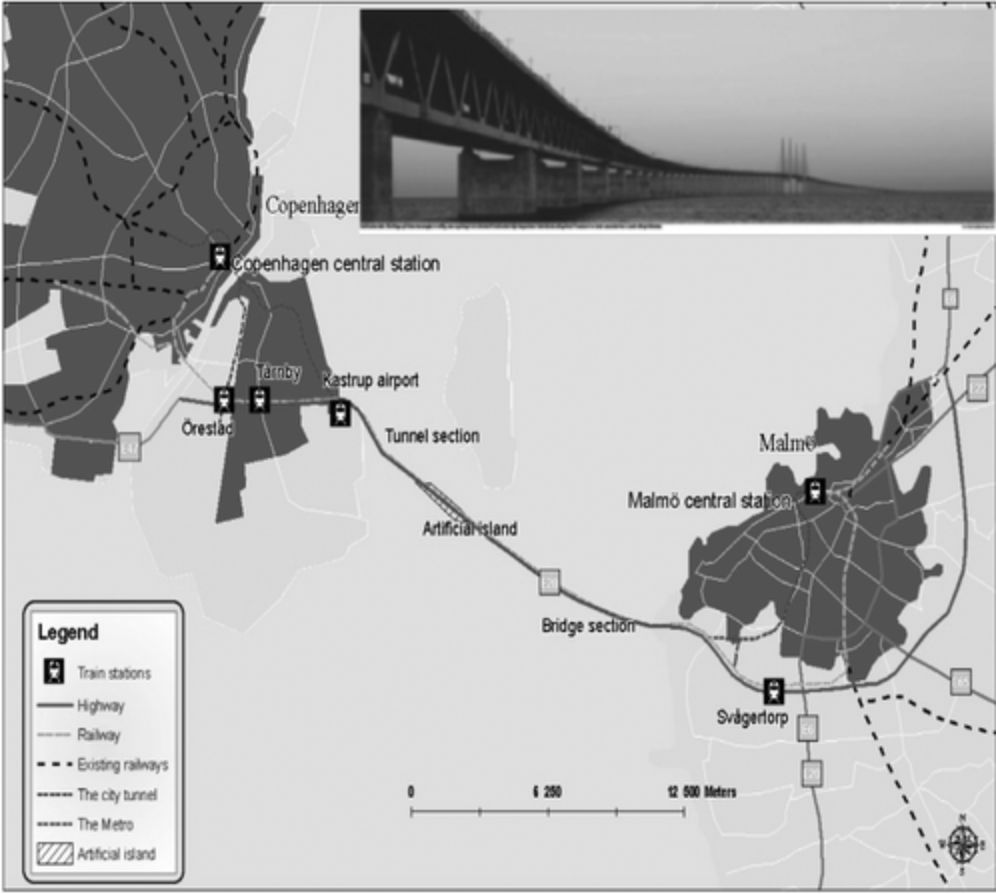
\includegraphics[width=0.7\linewidth,height=0.35\textheight]{figures/oresund.png}

\cite{khan2014constructive}

%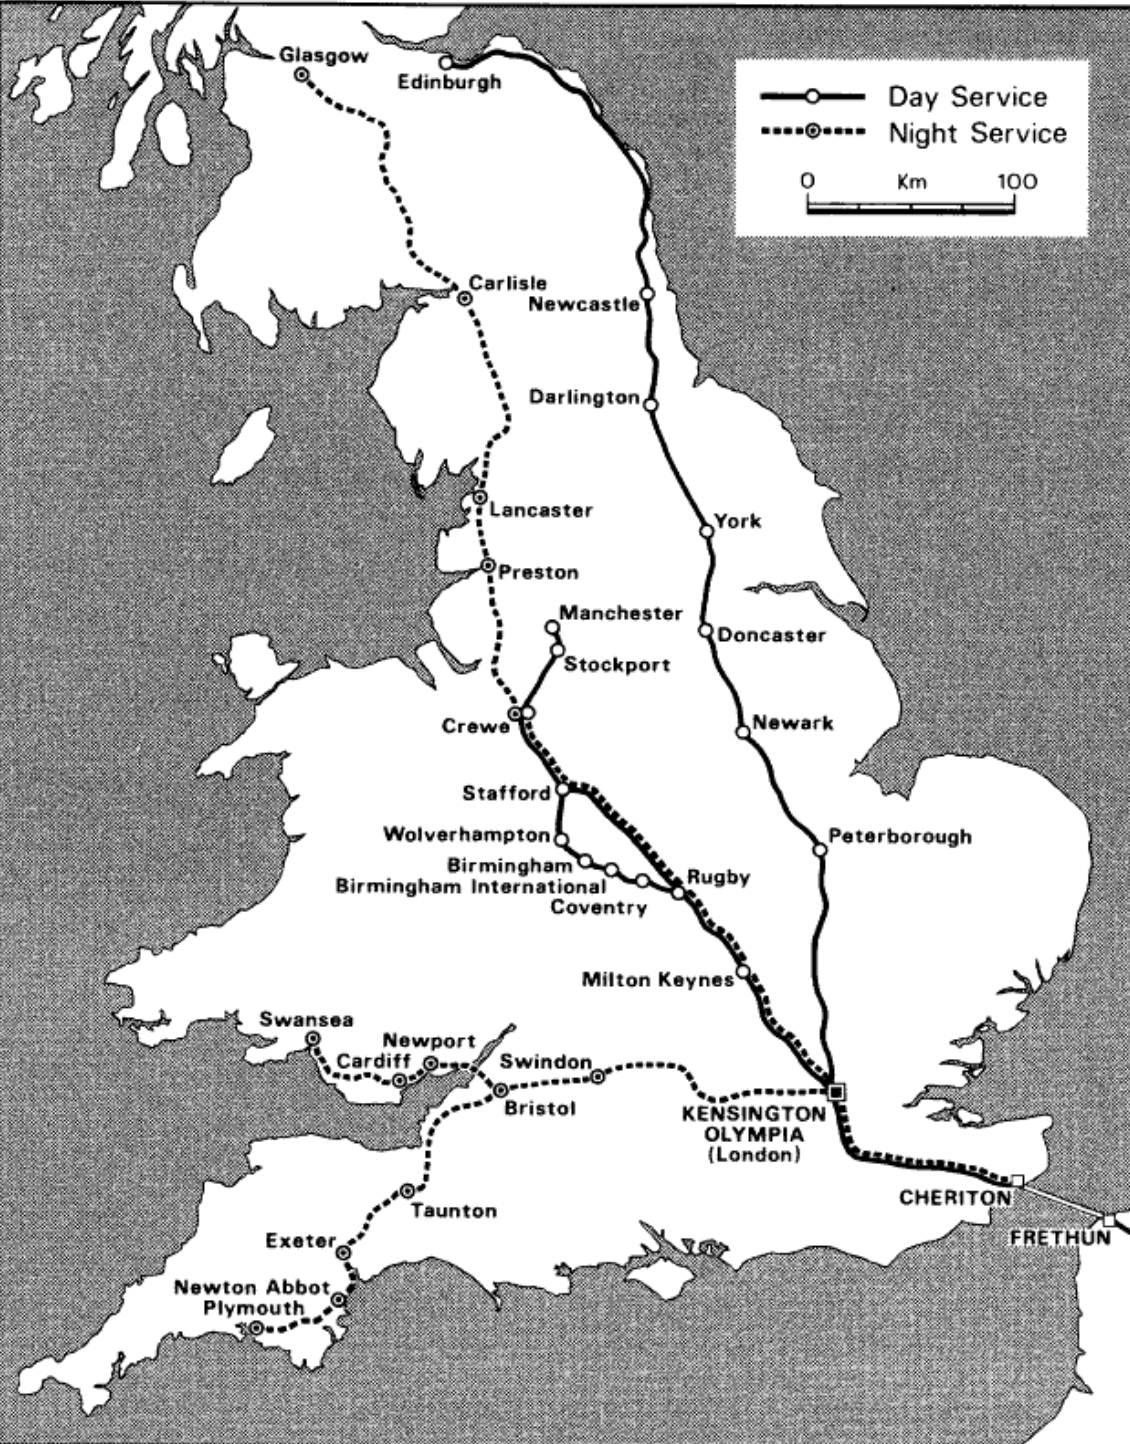
\includegraphics[width=0.5\linewidth]{figures/channeltunnel.png}

\cite{gibb1992channel}

%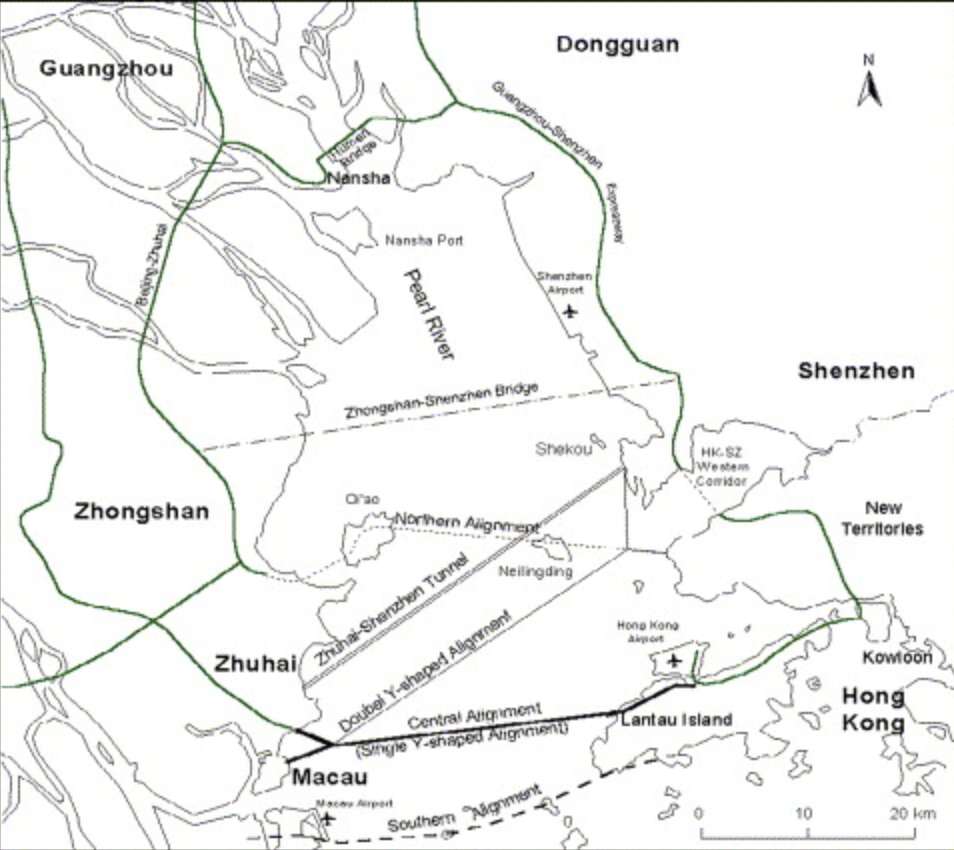
\includegraphics[width=0.7\linewidth,height=0.35\textheight]{figures/HZMB.png}


\cite{yang2006geopolitics}


%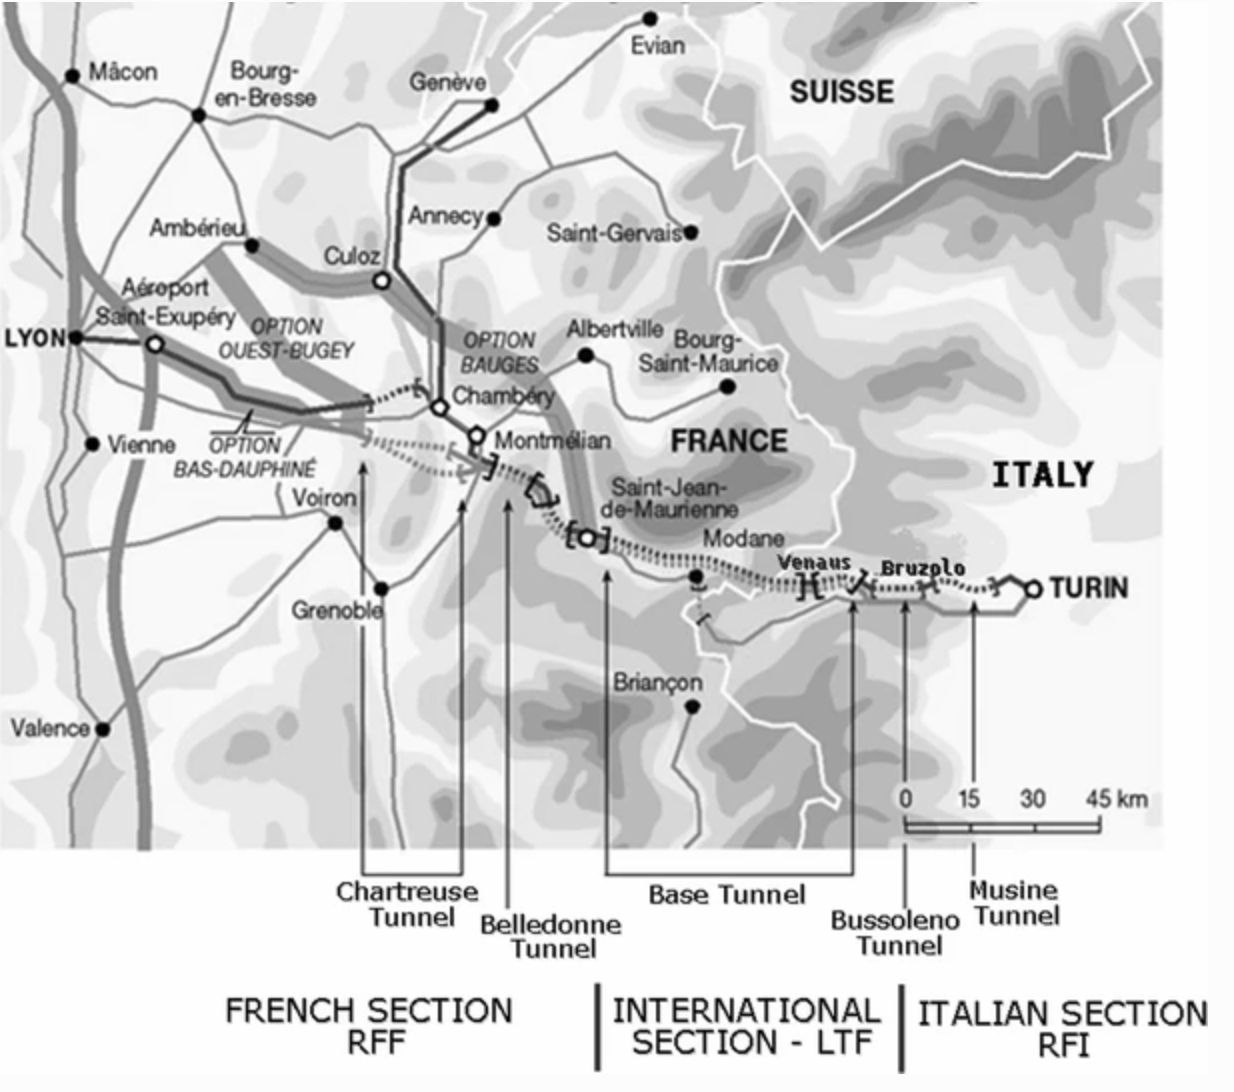
\includegraphics[width=0.7\linewidth]{figures/LyonTurin.png}

\cite{marincioni2009lyon}







Multinational transport investments

\textit{At the macroscopic scale: governance of multinational transport investments}


\begin{itemize}
	\item Positive effects of transport investments: \cite{melo2013productivity} meta-analysis, \cite{yii2018transportation} One-Belt-One-Road economic impact
	\item Difficult implementation of multinational investments \cite{tsamboulas1984multinational}; many trans-European projects fail in cost-benefit analysis \cite{proost2014selected} 
	\item Example of framework for prioritization based on multi-attribute theory \cite{tsamboulas2007tool}
\end{itemize}



Co-evolution and governance processes

\textbf{Modeling co-evolution with governance processes}



\begin{itemize}
	\item Model of governance choice \cite{Xie2011}
	\item Spatialized simulation model \cite{xie2011governance} 
	\item LUTI model with evolving network and game theory \cite{le2015modeling}
\end{itemize}



\textbf{Game theory and transportation models}


\begin{itemize}
	\item Competition HSR/airplane \cite{adler2010high} 
	\item Public-private partnerships \cite{medda2007game} 
	\item Public transport integration \cite{roumboutsos2008game}
\end{itemize}





Proposed approach

% Understanding such processes is crucial for sustainable planning at large scales. The issue of the interplay between bottom-up emergence of urban dynamics and top-down planning of infrastructures is in that context relevant to study. We propose in this contribution a model of co-evolution for cities and transportation networks, with a focus on how transportation networks evolve. More particularly, we extend the model of [3] by introducing top-down governance agents which decide on investments in transportation links.

% rq: have a look again at Mimeur's model


\textit{Interaction of bottom-up and top-down planning processes in network and territories co-evolution}

\medskip

 \textit{Stylized yet applicable simple models accounting for governance processes may be useful tools towards sustainable small scale territorial planning}
% rq: discussed - see review mesobench



\textbf{Research objective}

Explore a co-evolution model for cities and transportation networks at the macroscopic scale, focusing on network evolution rules including governance choices.







\section{Model}


Model rationale



% The model simulates population trajectories of cities and network link speed trajectories, with two main modules: (i) spatial interaction modeling to determine growth rates of cities, and (ii) governance modeling for network evolution.

$\rightarrow$ \textit{Extend the model of \cite{raimbault2020hierarchy} and \cite{raimbault2020modeling} with two governance levels (national and international) and the game theoretic cooperation module introduced by \cite{le2015modeling}}

\bigskip

\begin{itemize}
	\item Cities described by their population $P_i\left(t\right)$, linked with a physical transportation network with links described by effective distance $d_l\left(t\right)$
\end{itemize}
\begin{itemize}
	\item Iterative macro-scale LUTI simulation model: at each time step
		\begin{enumerate}
			\item Update spatial interaction flows
			\item Evolve cities populations depending on flows
			\item Evolve network speeds depending on link flows assigned in the network
		\end{enumerate}
\end{itemize}




Cities populations

%The model operates at the macroscopic scale: basic units are cities, distributed in space and described by their population $P_i$. A spatial interaction model is used to estimate flows between pairs of cities as

Spatial interaction flows

\[
\varphi_{ij} \textrm{=} \left( P_i P_j \right)^{\gamma} \cdot \exp\left(- \frac{d_{ij}}{d_0}\right)
\]

% From these flows is computed a growth rate for cities, assuming that it is for one city proportional to the sum of flows to all other cities, such that

\bigskip
\bigskip

Assume growth rate of cities are proportional to cumulated interaction flows as


\[
\frac{P_i \left(t \textrm{+} \Delta t\right) - P_i\left(t\right)}{\Delta t} \propto c_{ij} \cdot P_i\left(t\right)^{\gamma} \cdot \sum_j P_j\left(t\right)^{\gamma} \cdot \exp\left(- \frac{d_{ij}}{d_0}\right)
\]


with $c_{ij}$ a multiplier parameter equal to $1$ if cities are in the same country and $c_0 \leq 1$ otherwise

% WITH FIXED EFFECT COUNTRY MULTIPLIER

% Flows between cities are then distributed into the network. We assume no congestion and that the shortest path is taken.






Network


% Using a game-theoretic approach, macroscopic agents (such as governments or planning authorities) arbitrate stochastically between national and international investments, following a payoff-matrix considering optimal accessibility gains and collaboration costs, with probabilities obtained under the assumption of mixed strategies in a Nash equilibrium. Network investments are used to increase effective link speed by fixed increments.

%The set of deciders - which are the level of respective countries - evaluate the relevance of different infrastructure development options. More precisely, they have in a simplified setting the choice between an international collaboration and a strictly national infrastructure development. Let $Z^{\ast}_i$ be the optimal infrastructure in terms of accessibility gains for the country $i$ only, and $Z^{\ast}_C$ the optimal international infrastructure.
%Making the assumption that deciders aim at optimizing the accessibility gain, 

% - distinguish between national and international flows
% - link increase function: flow quantile, improve only if above (no decrease)


\begin{enumerate}
	\item Baseline model: self-reinforcment of link speed according to
	\[
	d_l\left(t \textrm{+} \Delta t\right) \textrm{=} d_l\left(t\right) \cdot \left[ 1 \textrm{+} \Delta t \cdot g_M \left( \frac{1 - \left(\frac{\varphi_l}{\varphi_0}\right)^{\gamma_N}}{1 \textrm{+} \left(\frac{\varphi_l}{\varphi_0}\right)^{\gamma_N}} \right) \right]	
	\]
	for links with $\varphi_l > \varphi_0$, where $\varphi_0$ corresponds to the $\varphi_0^{(q)}$ quantile of link flows
	\item Estimate for each country $k$ accessibility gains $\Delta Z_k^{(N)}$ and $\Delta Z_k^{(I)}$ obtained respectively with national $(N)$ and international $(I)$ flows, and corresponding construction costs $C_k^{(N)}$, $C_k^{(I)}$
\end{enumerate}




Payoff matrix

Utility matrix for the two actor game is



\begin{table}
\begin{tabular}{|c|c|c|} 
 \hline
 0 $|$ 1  & C & NC \\ \hline
 C & $U_i = \Delta Z_k^{(I)} - \kappa \cdot C_k^{(I)} - \frac{J}{2}$
   & $\begin{cases} U_0 = \Delta Z_0^{(N)} - \kappa \cdot C_0^{(N)} \\U_1 = \Delta Z_1^{(N)} - \kappa \cdot C_1^{(N)} - \frac{J}{2}\end{cases}$ \\ \hline
 NC & $\begin{cases}U_0 = \Delta Z_0^{(N)} - \kappa \cdot C_0^{(N)} - \frac{J}{2}\\U_1 = \Delta Z_1^{(N)} - \kappa \cdot C_1^{(N)}\end{cases}$
   & $U_i =  \Delta Z_i^{(N)} - \kappa \cdot C_i^{(N)}$ \\
 \hline
\end{tabular}
\end{table}



Mixed Nash equilibrium probabilities

The general mixed Nash equilibrium probabilities are

\medskip

\[
p_{1-i} = - \frac{U_i\left(C,NC\right) - U_i\left(NC,NC\right)}{\left(U_i\left(C,C\right) - U_i\left(NC,C\right)\right) - \left(U_i\left(C,NC\right) - U_i\left(NC,NC\right)\right)}
\]



what gives with the payoff matrix



\[
p_i \textrm{=} \frac{J}{\left(Z_{1-i}^{(I)} - Z_{1-i}^{(N)}\right) - \kappa \cdot \left(C_{1-i}^{(I)} - C_{1-i}^{(N)}\right)}
\]

% from lutecia paper
% It also forces feasibility conditions on $J$ and accessibility gains to keep a probability. These are
%\begin{itemize}
%	\item $ J \leq \Delta X_{1 - i}(Z^{\star}_{C}) - \Delta X_{1 - i}(Z^{\star}_{1 - i})$, what can be interpreted as a cost-benefits condition for cooperation, e.g. that the gain induced by the common infrastructure must be larger than the collaboration cost;
%	\item $\Delta X_{1 - i}(Z^{\star}_{C}) \leq \Delta X_{1 - i}(Z^{\star}_{1 - i})$, e.g. that the gain induced by the common infrastructure must be positive.
%\end{itemize}


% ! non collab game? justify? // other approach such as DC?


Parameters $\kappa, J$ are in practiced rescaled such that: (i) given a baseline model run, average cost absolute difference times $\kappa$ is a fixed proportion $k_0$ of average absolute accessibility difference; and (ii) collaboration cost $J$ yields a fixed probability $p_0$ computed on absolute average of the baseline run.






\section{Results}

Implementation and experiments

% The model is applied to synthetic systems of cities, in a stylized configuration of two neighbor countries of comparable size. We systematically study model behavior with the OpenMOLE platform for model exploration and validation [4].



\textbf{Implementation}

\begin{itemize}
	\item Model implemented in NetLogo (good compromise interactivity / ergonomy), with fast data structures (matrix/table extensions)
	\item Applied on synthetic systems of cities \cite{raimbault2019second}
	\item Integrated seamlessly into OpenMOLE \cite{reuillon2013openmole} for model exploration \url{https://openmole.org/}
\end{itemize}

%\begin{center}
%
\includegraphics[width=0.1\linewidth]{figures/iconOM.png}
%
\includegraphics[width=0.4\linewidth]{figures/openmole.png}
%\end{center}



\textbf{Experiments}

\begin{itemize}
	\item Saltelli Global Sensitivity Analysis \cite{saltelli2008global}
	\item Role of stochasticity
	\item Grid experiment with role of spatial configuration
\end{itemize}



\paragraph{Example of simulated systems}{
 
%\begin{center}
%	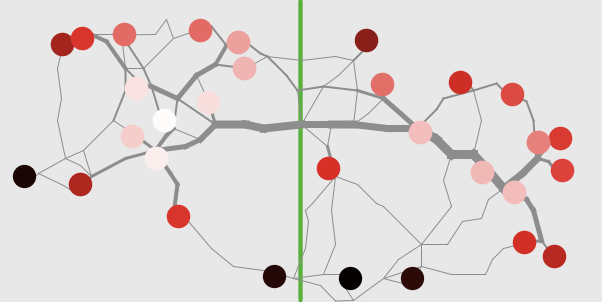
\includegraphics[width=0.65\linewidth]{figures/ex_baseline.png}\\\hrule
%	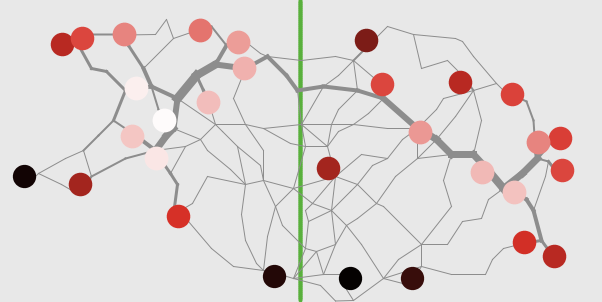
\includegraphics[width=0.65\linewidth]{figures/ex_baseline_full.png}
%\end{center}

 
 


\paragraph{Global sensitivity analysis}

% First exploration results suggest a strong qualitative influence of propensity to collaborate on trajectories of the full system

% first order
% deltaPop,
%deltaAccessibility,
%deltaHierarchiesPop,
% rankCorrPop,
% governanceLevel,
%networkCost,

% total order

% ,,,,,,,,,
%deltaAccessibility,
% deltaHierarchiesPop,
% rankCorrPop,
% governanceLevel,
% networkCost,

% synthRankSize,gravityGamma,gravityDecay,gravityInterRatio,nwGmax,nwExponent,nwReinQuantile,govCostToAccess,govEffectiveProba,seed



\textbf{Indicators: } $\Delta P$ average population growth; $\Delta Z$ average accessibility growth; $\Delta \alpha_P$ population hierarchy change; $r_P$ population rank correlation; $g$ average governance level; $C$ total cost


\begin{table}
\resizebox{\linewidth}{!}{
    \begin{tabular}{|l|c|c|c|c|c|c|c|c|c|c|c|c|c|c|c|c|c|c|c|c|}
\hline
 & \multicolumn{2}{|c|}{$\alpha_0$} & \multicolumn{2}{|c|}{$\gamma_G$} & \multicolumn{2}{|c|}{$d_G$} & \multicolumn{2}{|c|}{$c_0$} & \multicolumn{2}{|c|}{$g_{max}$} & \multicolumn{2}{|c|}{$\gamma_N$}  & \multicolumn{2}{|c|}{$\varphi_0^{(q)}$}  & \multicolumn{2}{|c|}{$k_0$} & \multicolumn{2}{|c|}{$p_0$} & \multicolumn{2}{|c|}{$S$} \\
 & F & T & F & T & F & T & F & T & F & T & F & T & F & T & F & T & F & T & F & T \\
 \hline
$\Delta P$ & 0.094 & 0.22 & 0.17 & 0.37 & 0.07 & 0.15 & 0.3 & 0.59 & $7\cdot 10^{-5}$ & 0.003 & -0.002 & $6.9\cdot 10^{-4}$ & -0.002 & 0.002 & -0.001 & 0.0003 & 0.002 & 0.003 & 0.02 & 0.06 \\
$\Delta Z$ & 0.05 & 0.1 & 0.02 & 0.16 & 0.52 & 0.8 & 0.02 & 0.03 & -0.006 & 0.18 & -0.006 & 0.008 & -0.008 & 0.03 & 0.0005 & 0.003 & -0.006 & 0.01 & -0.005 & 0.1 \\
$\Delta \alpha_P$ & 0.2 & 0.3 & 0.3 & 0.5 & 0.06 & 0.12 & 0.17 & 0.26 & -0.002 & 0.002 & 0.0001 & 0.0003 & -0.004 & 0.001 &-0.0007 & 0.0003 & - 0.0008 & 0.0008 & 0.01 & 0.04 \\
$r_P$ & -0.7& 0.1 & -0.1& 0.2 &-0.4 & 0.3& 0.26& 0.002 & -0.09 & 0.01 & 0.5 & 0.01 & 1.0 & 0.09 & 0.1 & 0.0002 & 0.3 & 0.001 & 0.1 & 0.07 \\
$g$ & -0.01 & 0.26 & -0.004 & 0.3 & -0.01 & 0.44 &0.03 & 0.6 & -0.03& 0.25 &-0.02 &0.2 & -0.05 & 0.3 & -0.01 & 0.2 & 0.07 & 0.7 & -0.01 & 0.5 \\
$C$ & -0.002 & 0.002 &-0.007 & 0.01 & -0.001& 0.002 & 0.002 & 0.002 & 0.06 &0.09 & 0.002 & 0.01 &0.8 & 0.9 & -0.0008 & 0.0005 &0.003 & 0.003 & 0.04& 0.04 \\\hline
\end{tabular}
}
\end{table}


\textit{effect of spatial configuration (seed and hierarchy) \cite{raimbault2019space}; 
crossed effects between network, cities and governance}

% + stat analysis? later



\paragraph{Role of stochasticity}

On 100 parameters sampled (LHS) with 100 replications:

\begin{itemize}
	\item All indicators have a high Sharpe ratio (1st quartile with a minimum of 7.7 expect governance level $g$ with a median at 1.02)
	\item Distance between average relative to standard deviations are also high (1st quartile higher than 2.3, except for $g$ with a median at 1.2 and $r_P$ with a median of 1.26)
\end{itemize}

%\medskip

%\begin{center}
%	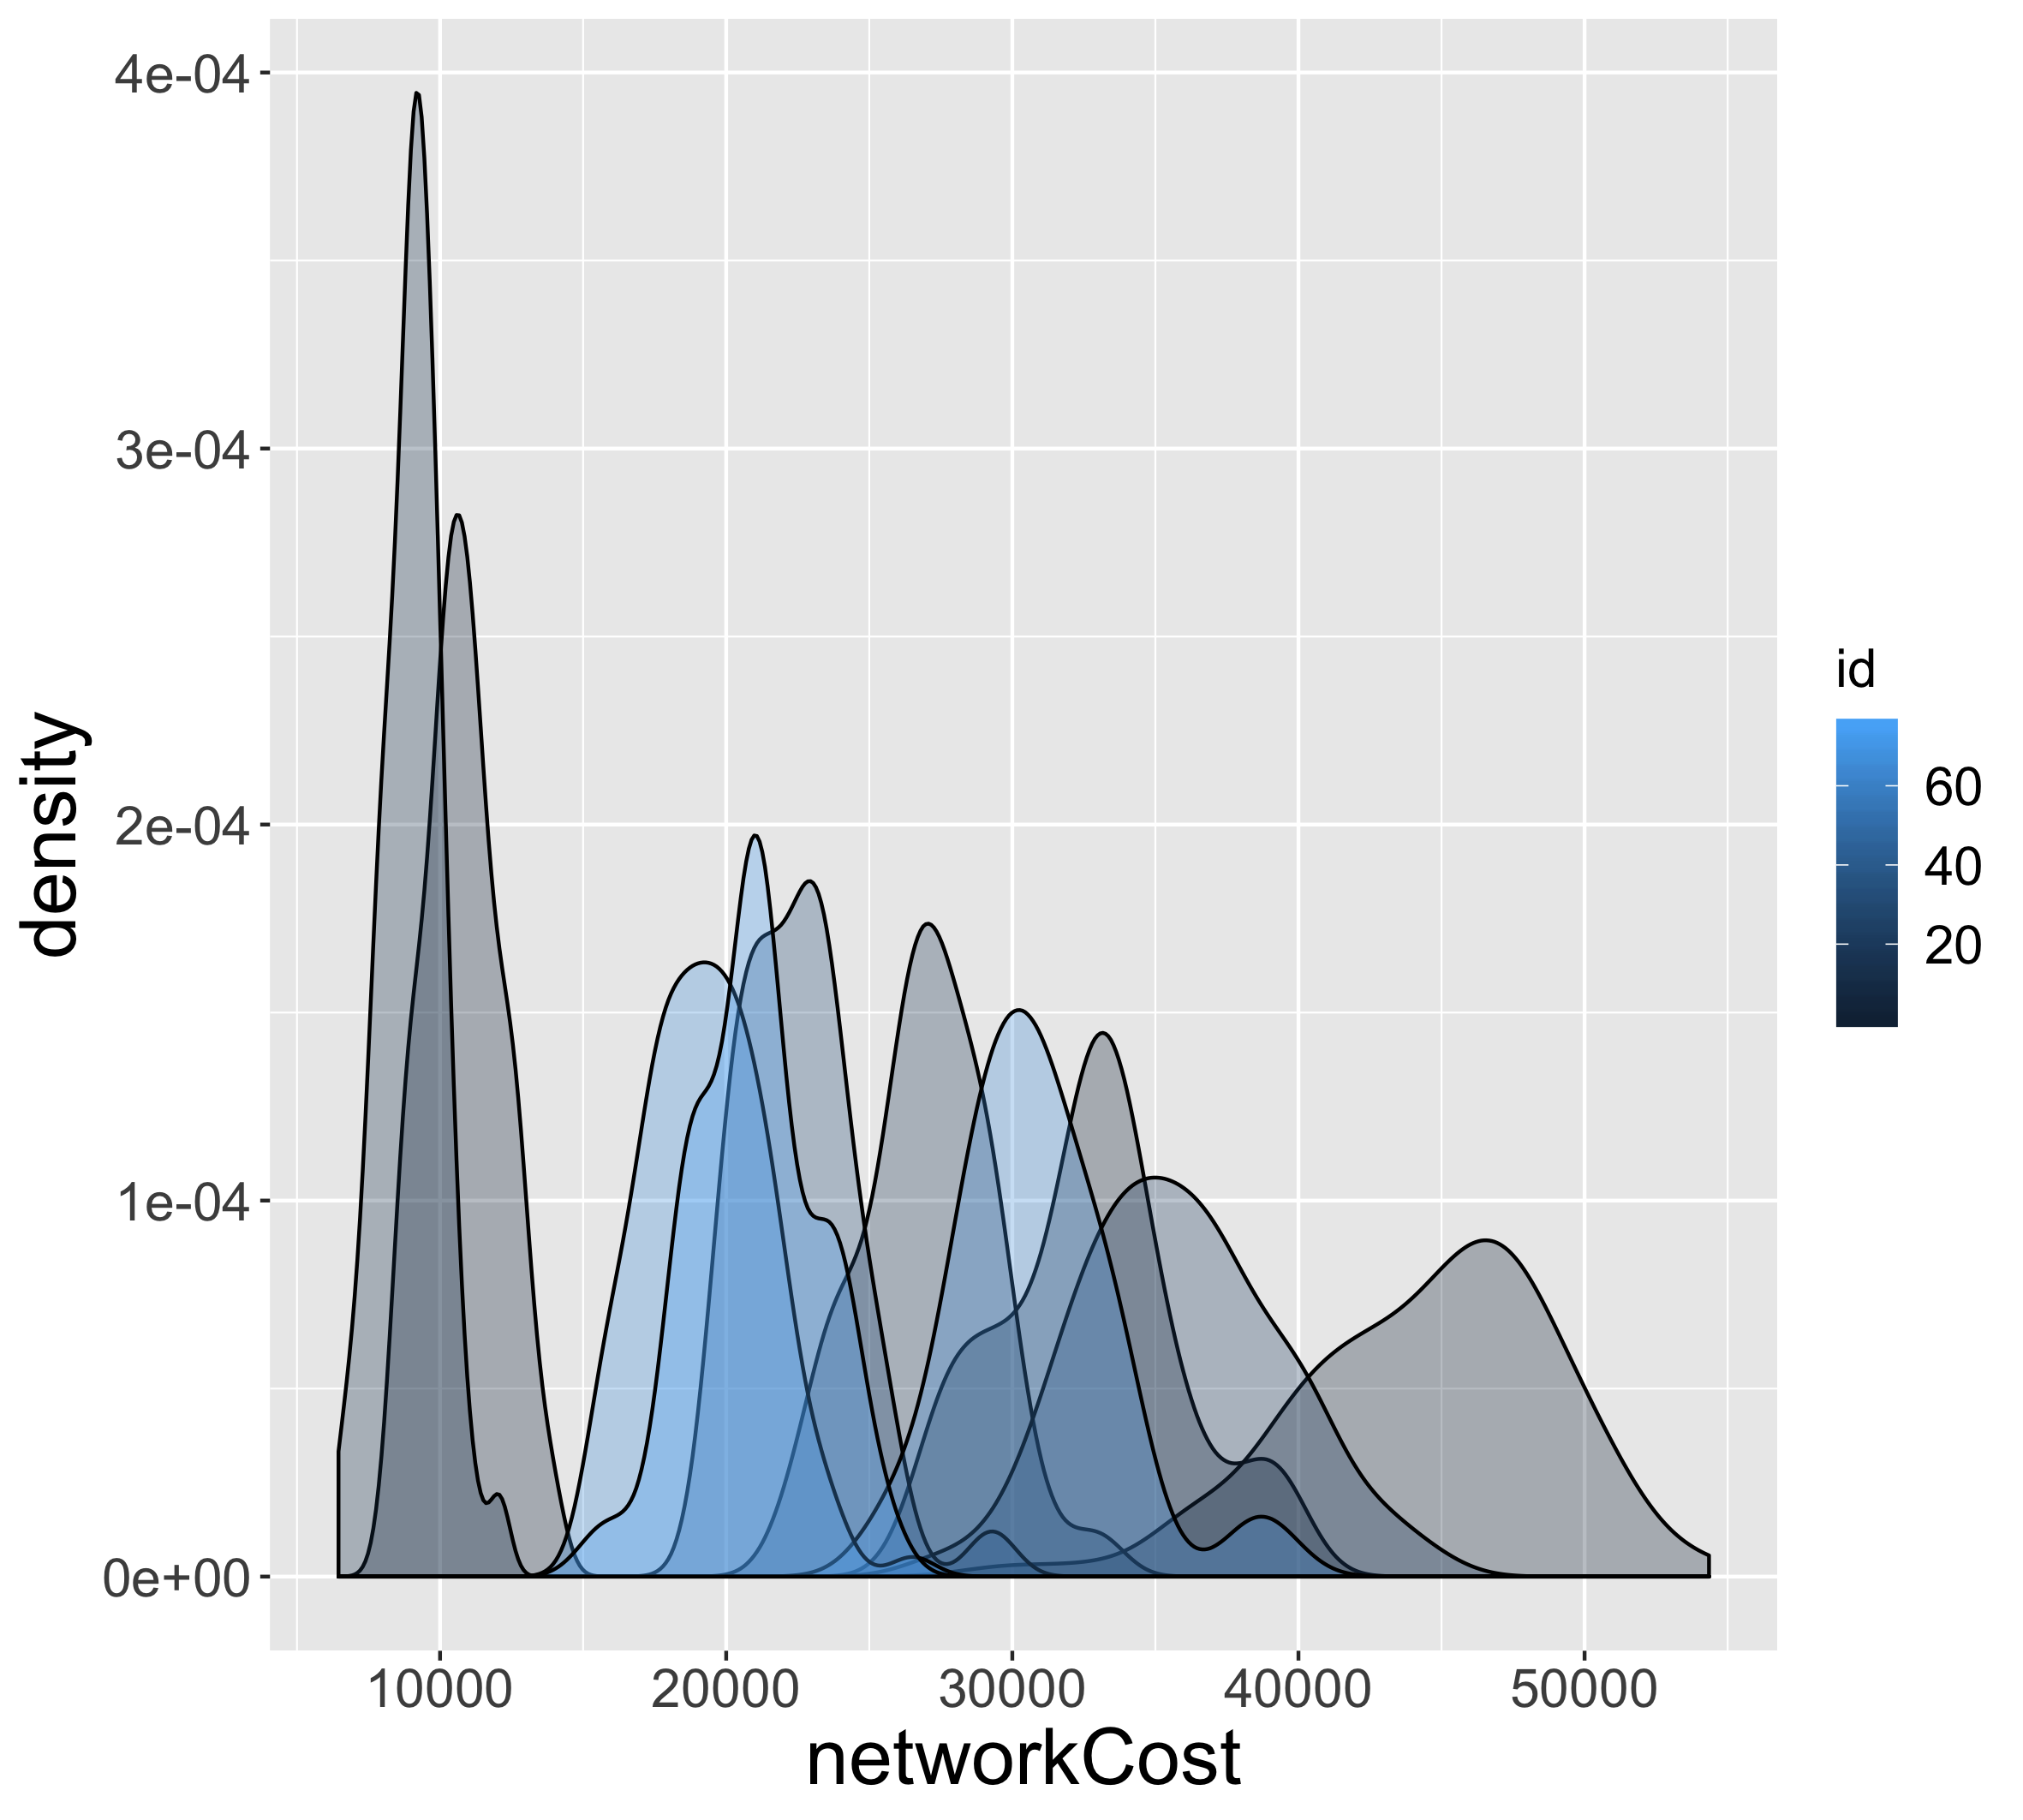
\includegraphics[width=0.4\textwidth]{figures/networkCost_samples10-seed42.png}
%	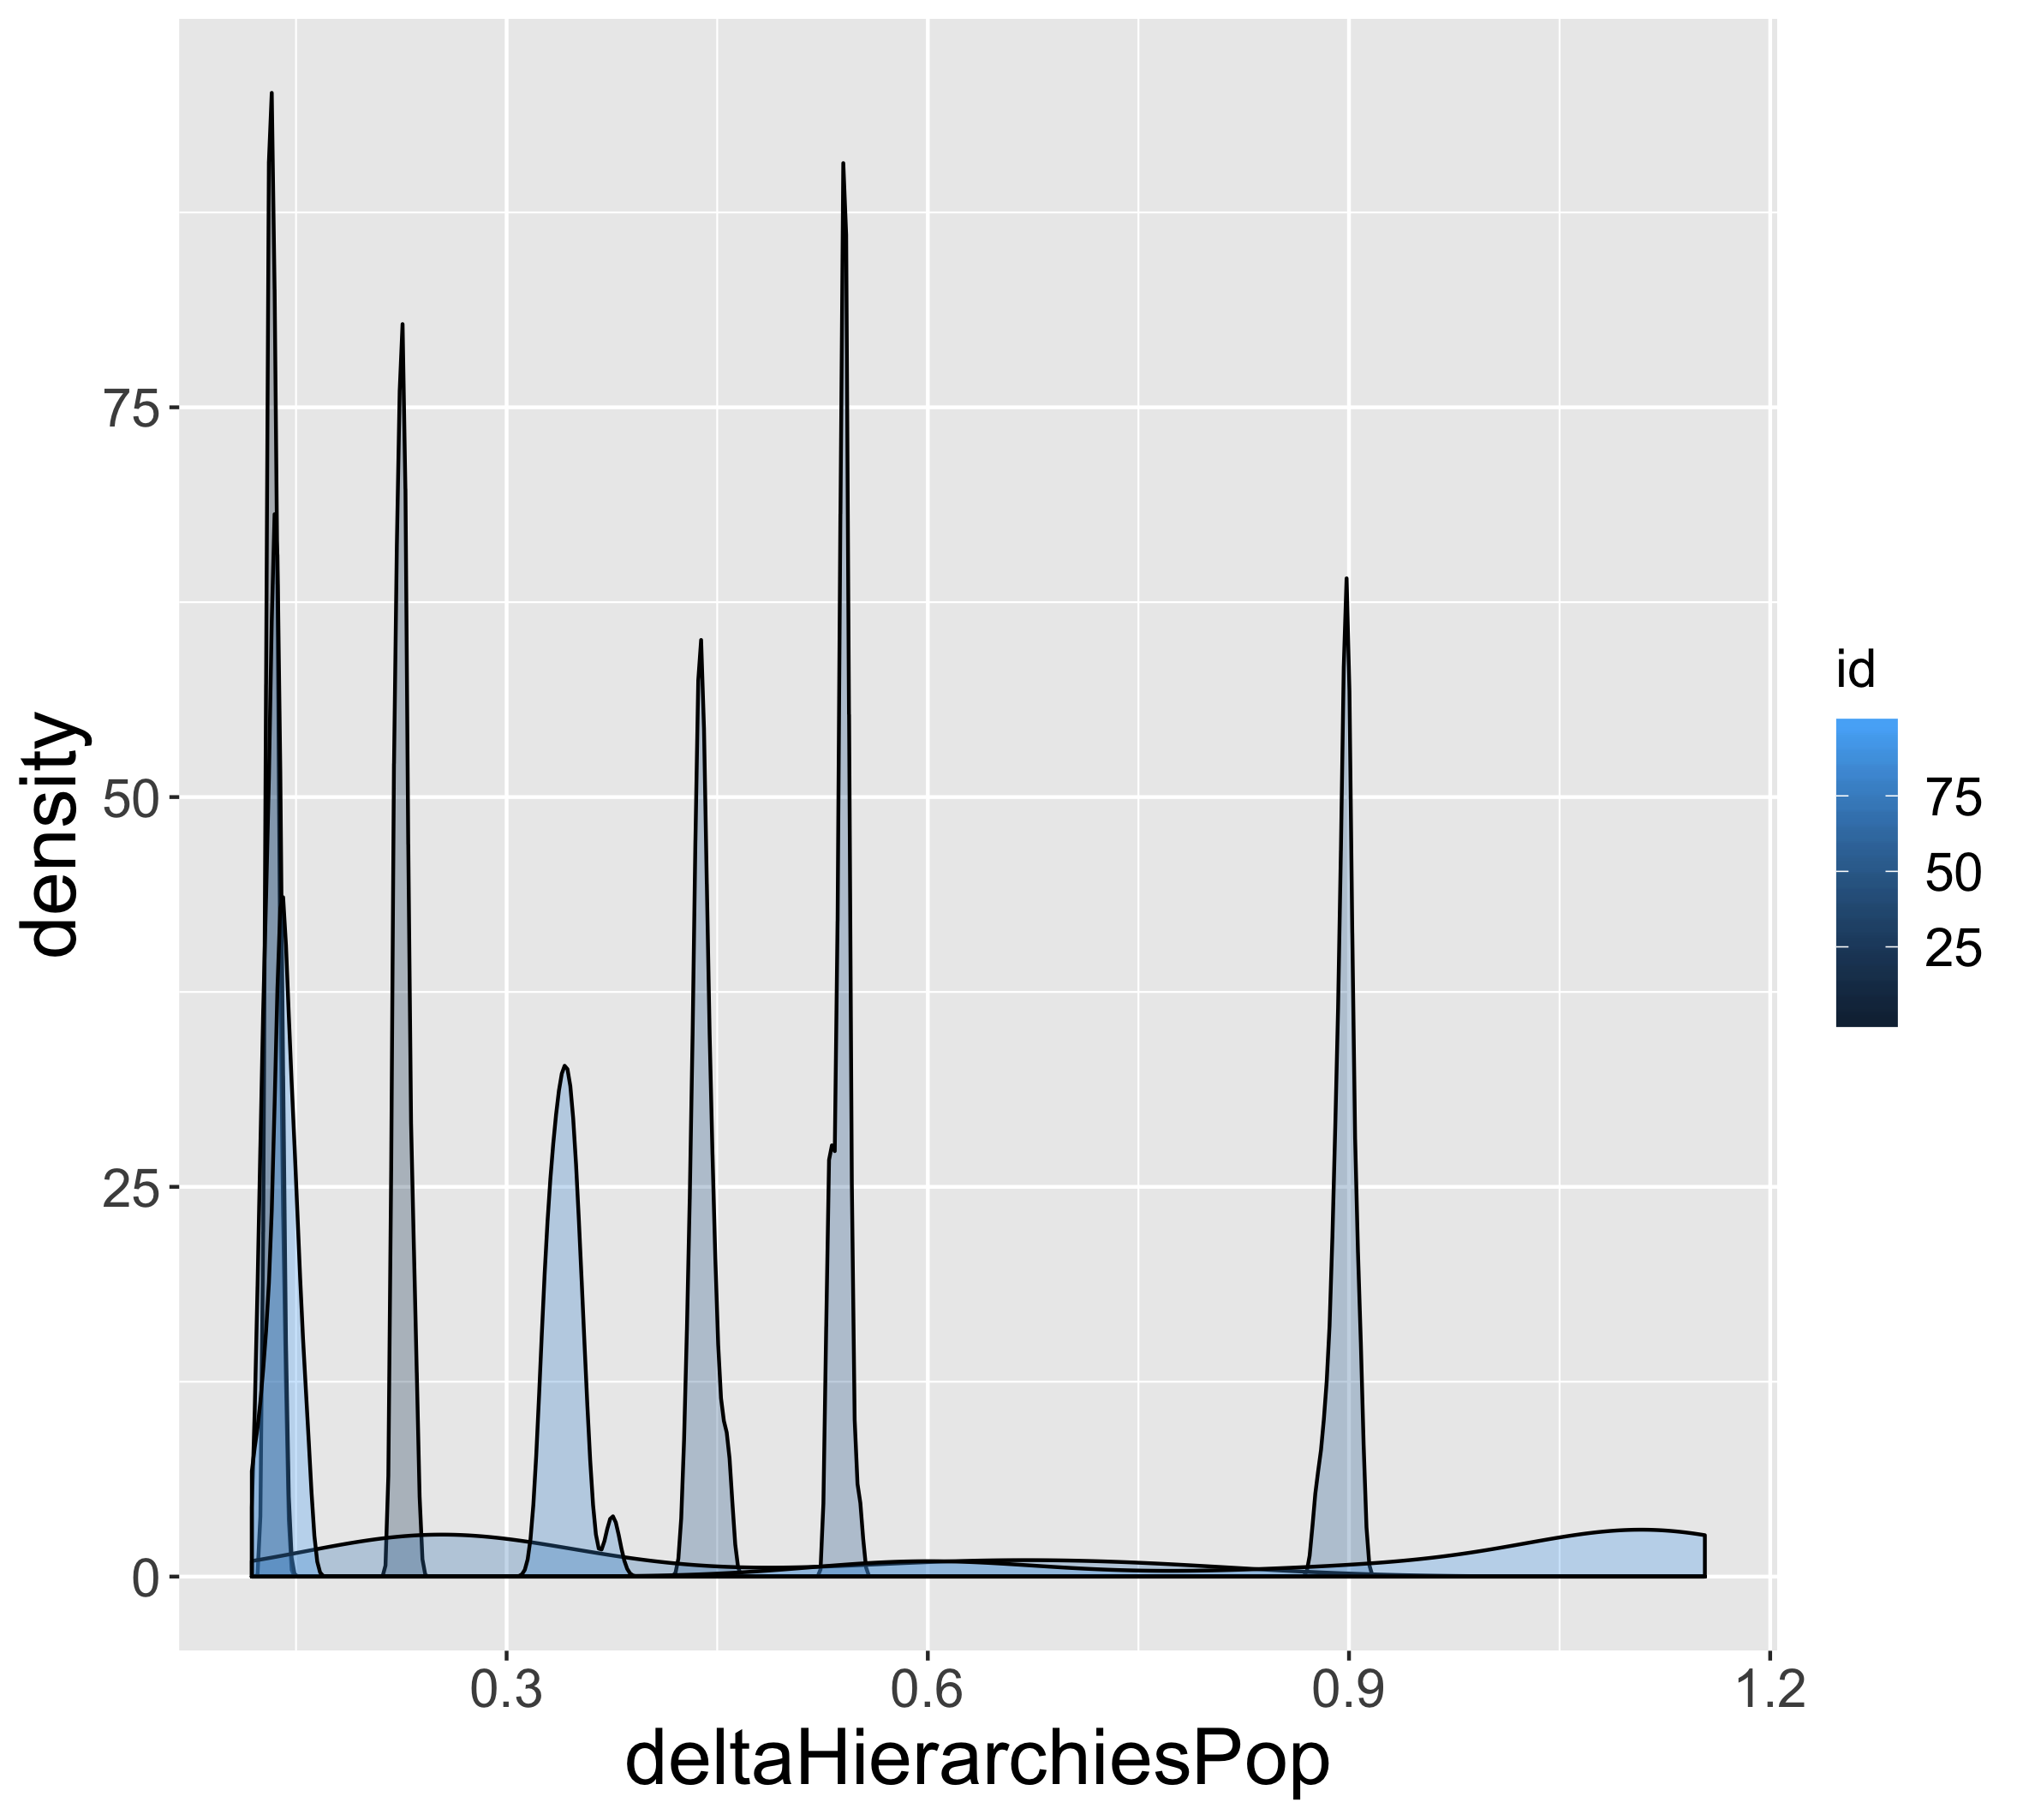
\includegraphics[width=0.4\textwidth]{figures/deltaHierarchiesPop_samples10-seed666.png}
%\end{center}






\paragraph{Grid exploration}

% , and that intermediate levels of international investments may be more optimal in terms of accessibility gains at fixed costs. In comparison to null model behavior obtained running the base model from [3], the introduction of top-down governance decisions also changes considerably model behavior.

% pareto fronts?
% grid plot for some indicators.




%\begin{center}
%	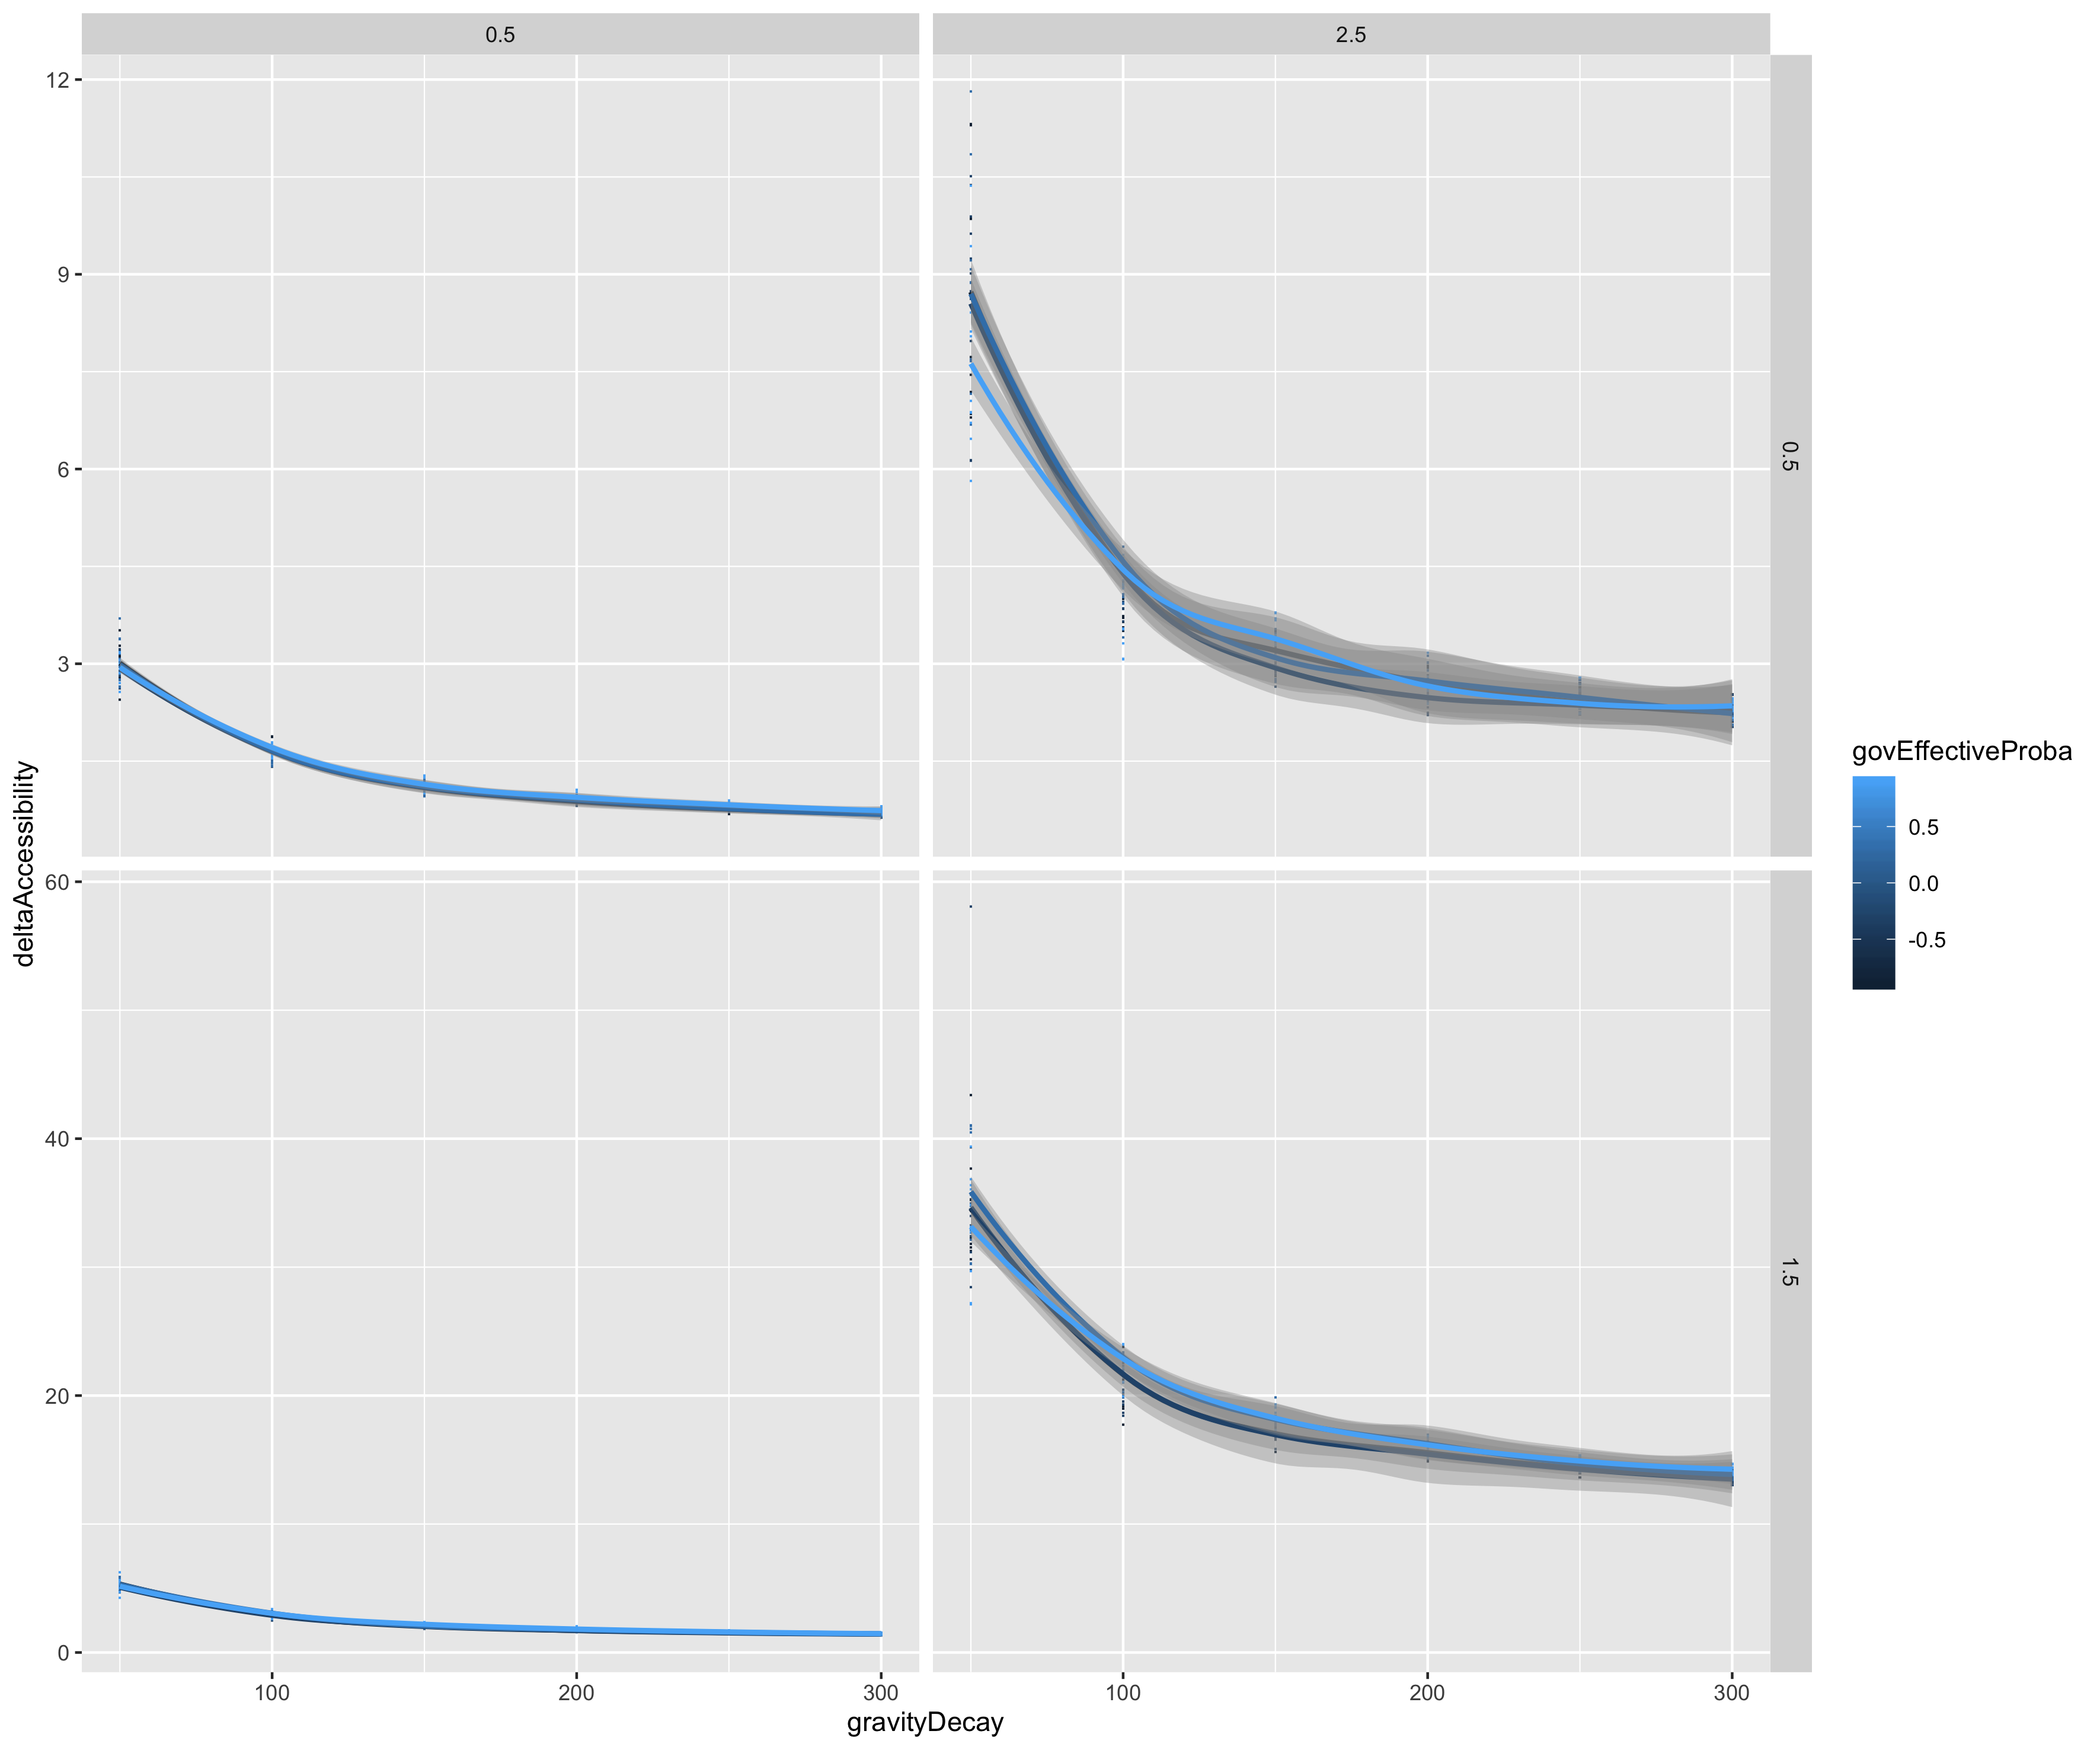
\includegraphics[width=0.5\textwidth]{figures/deltaAccessibility_gravityInterRatio0_75_govCostToAccess0_75_nwExponent2_nwGmax0_05_nwReinQuantile0_1.png}
%	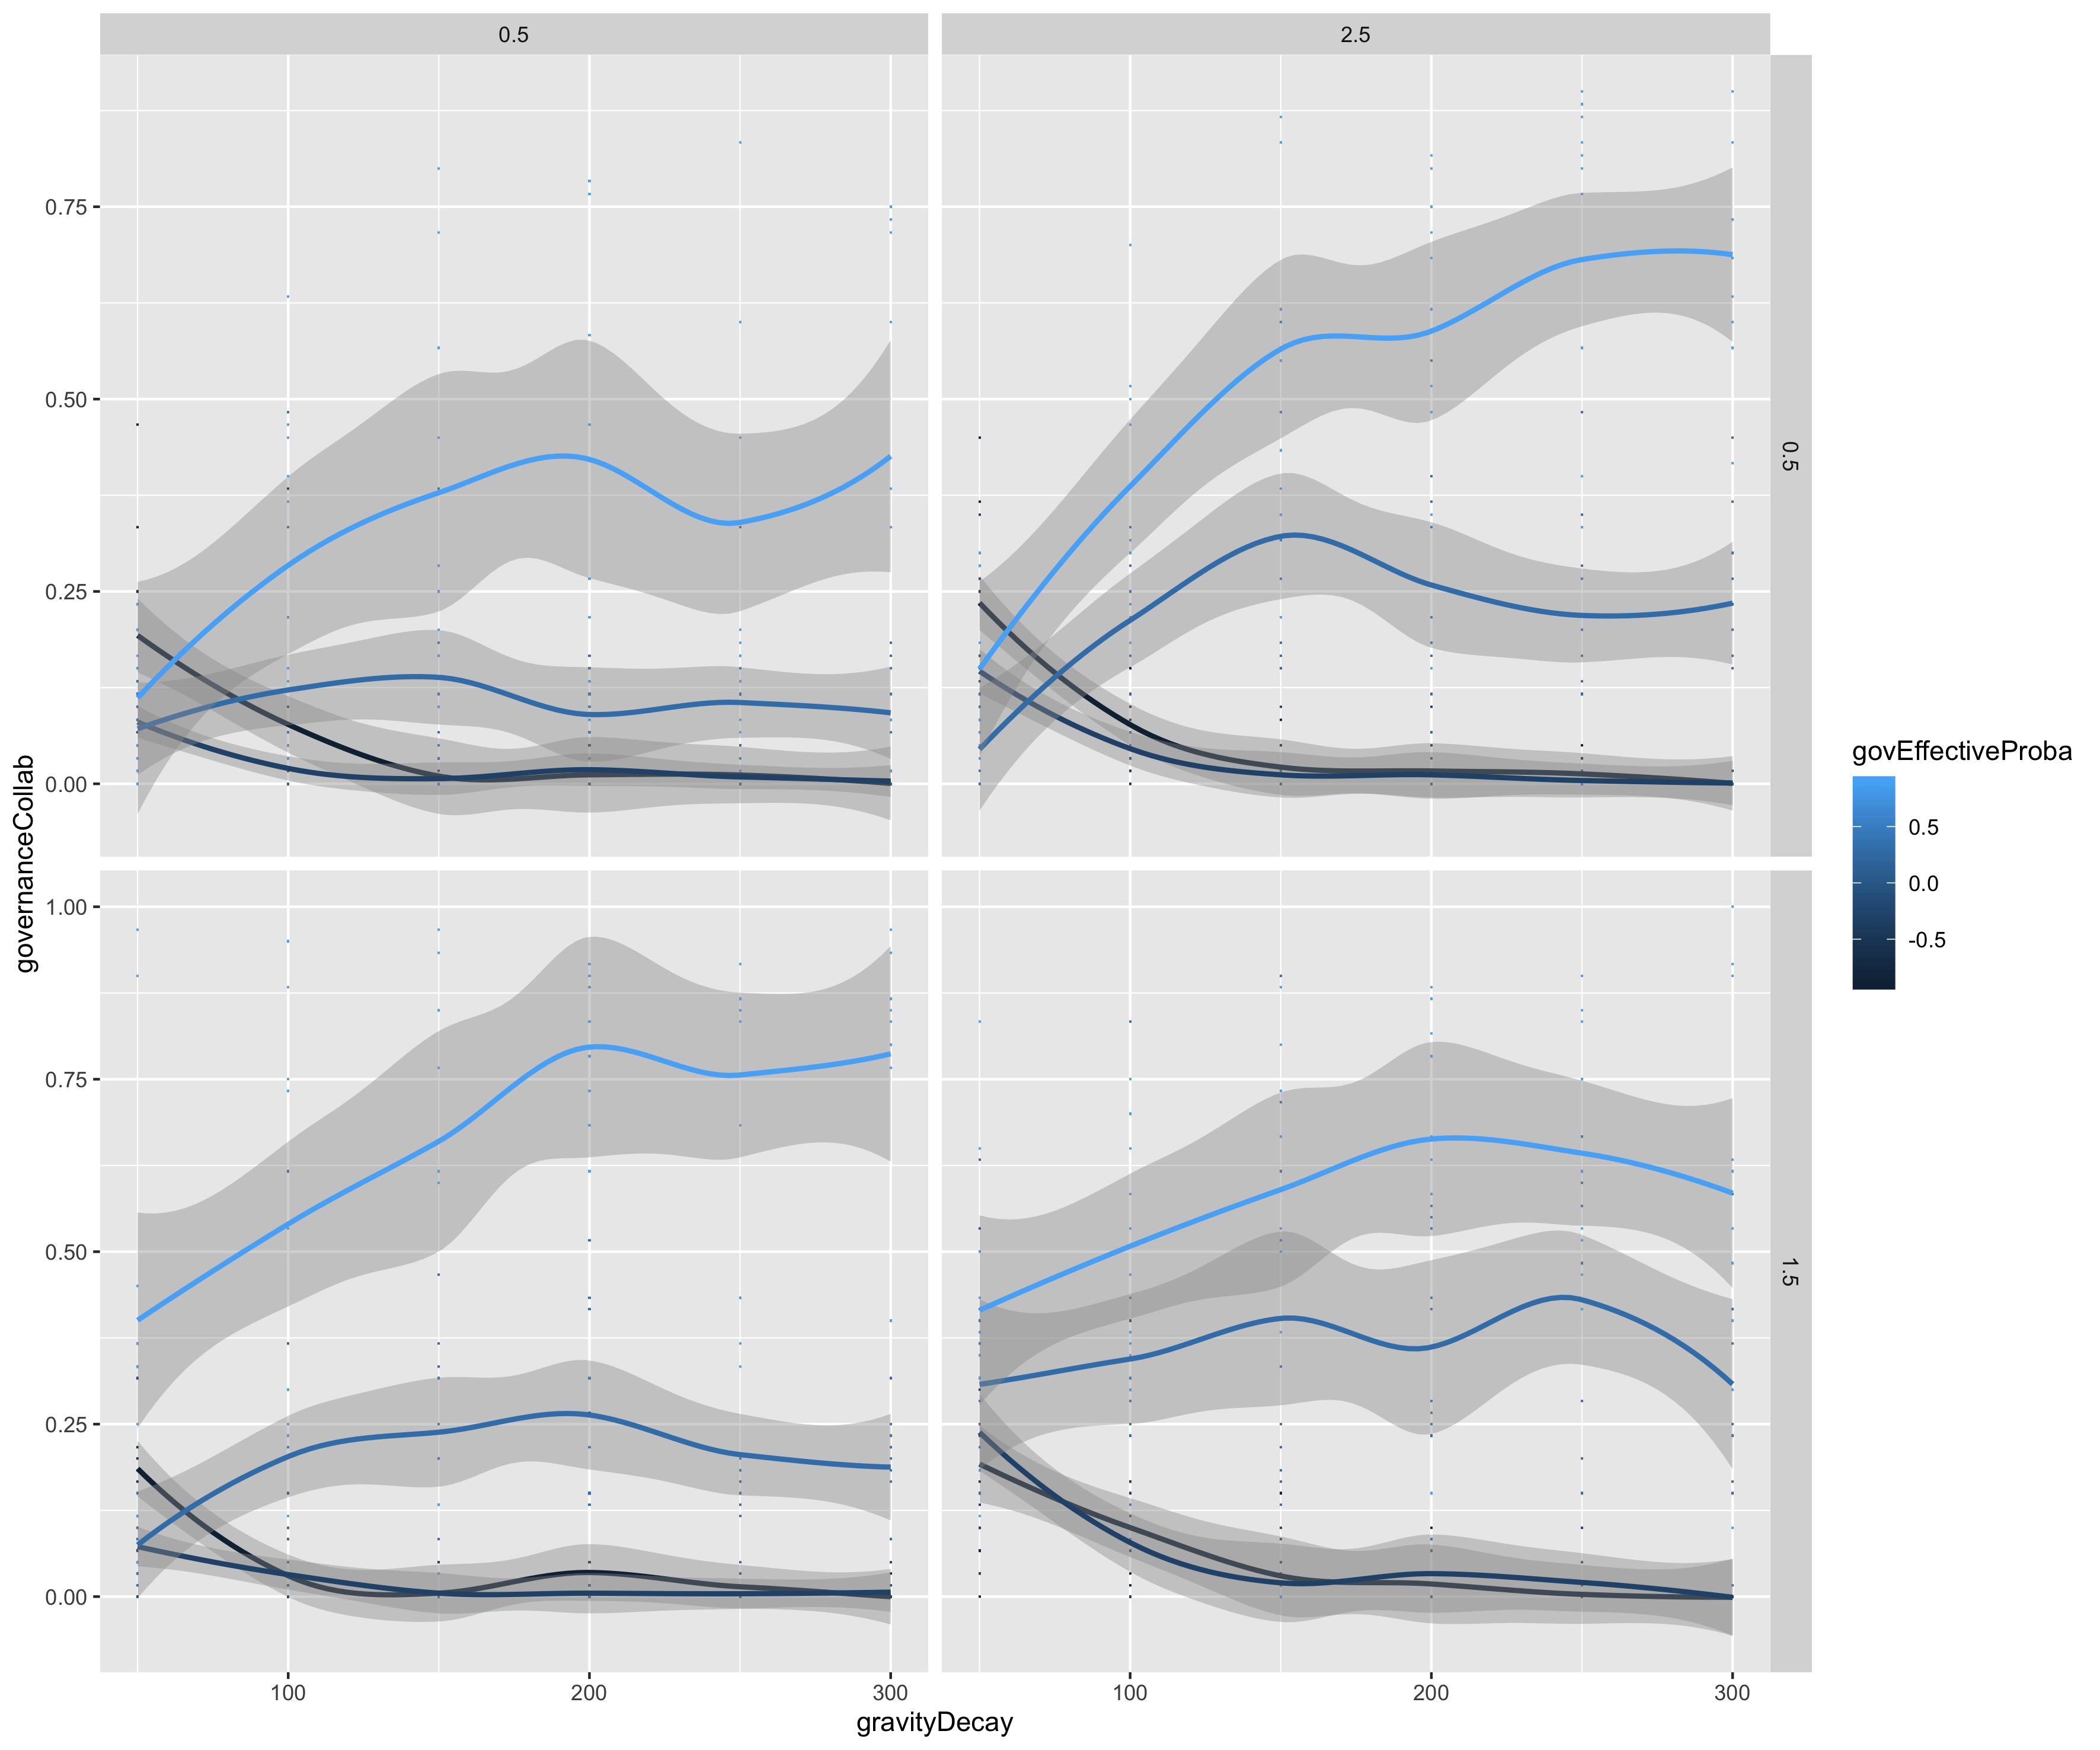
\includegraphics[width=0.5\textwidth]{figures/governanceCollab_gravityInterRatio0_75_govCostToAccess0_25_nwExponent2_nwGmax0_05_nwReinQuantile0_1.png}
%\end{center}

{\footnotesize Rows: hierarchy; columns: $\gamma_G$}

\textit{Larger span in spatial interaction decrease relative accessibility gain, as do less hierarchical flows; effect of interaction decay on governance level qualitatively changed by $p_0$}




\paragraph{Optimizing accessibility and cost}

% TODO figures in eps format
%\begin{figure}
%	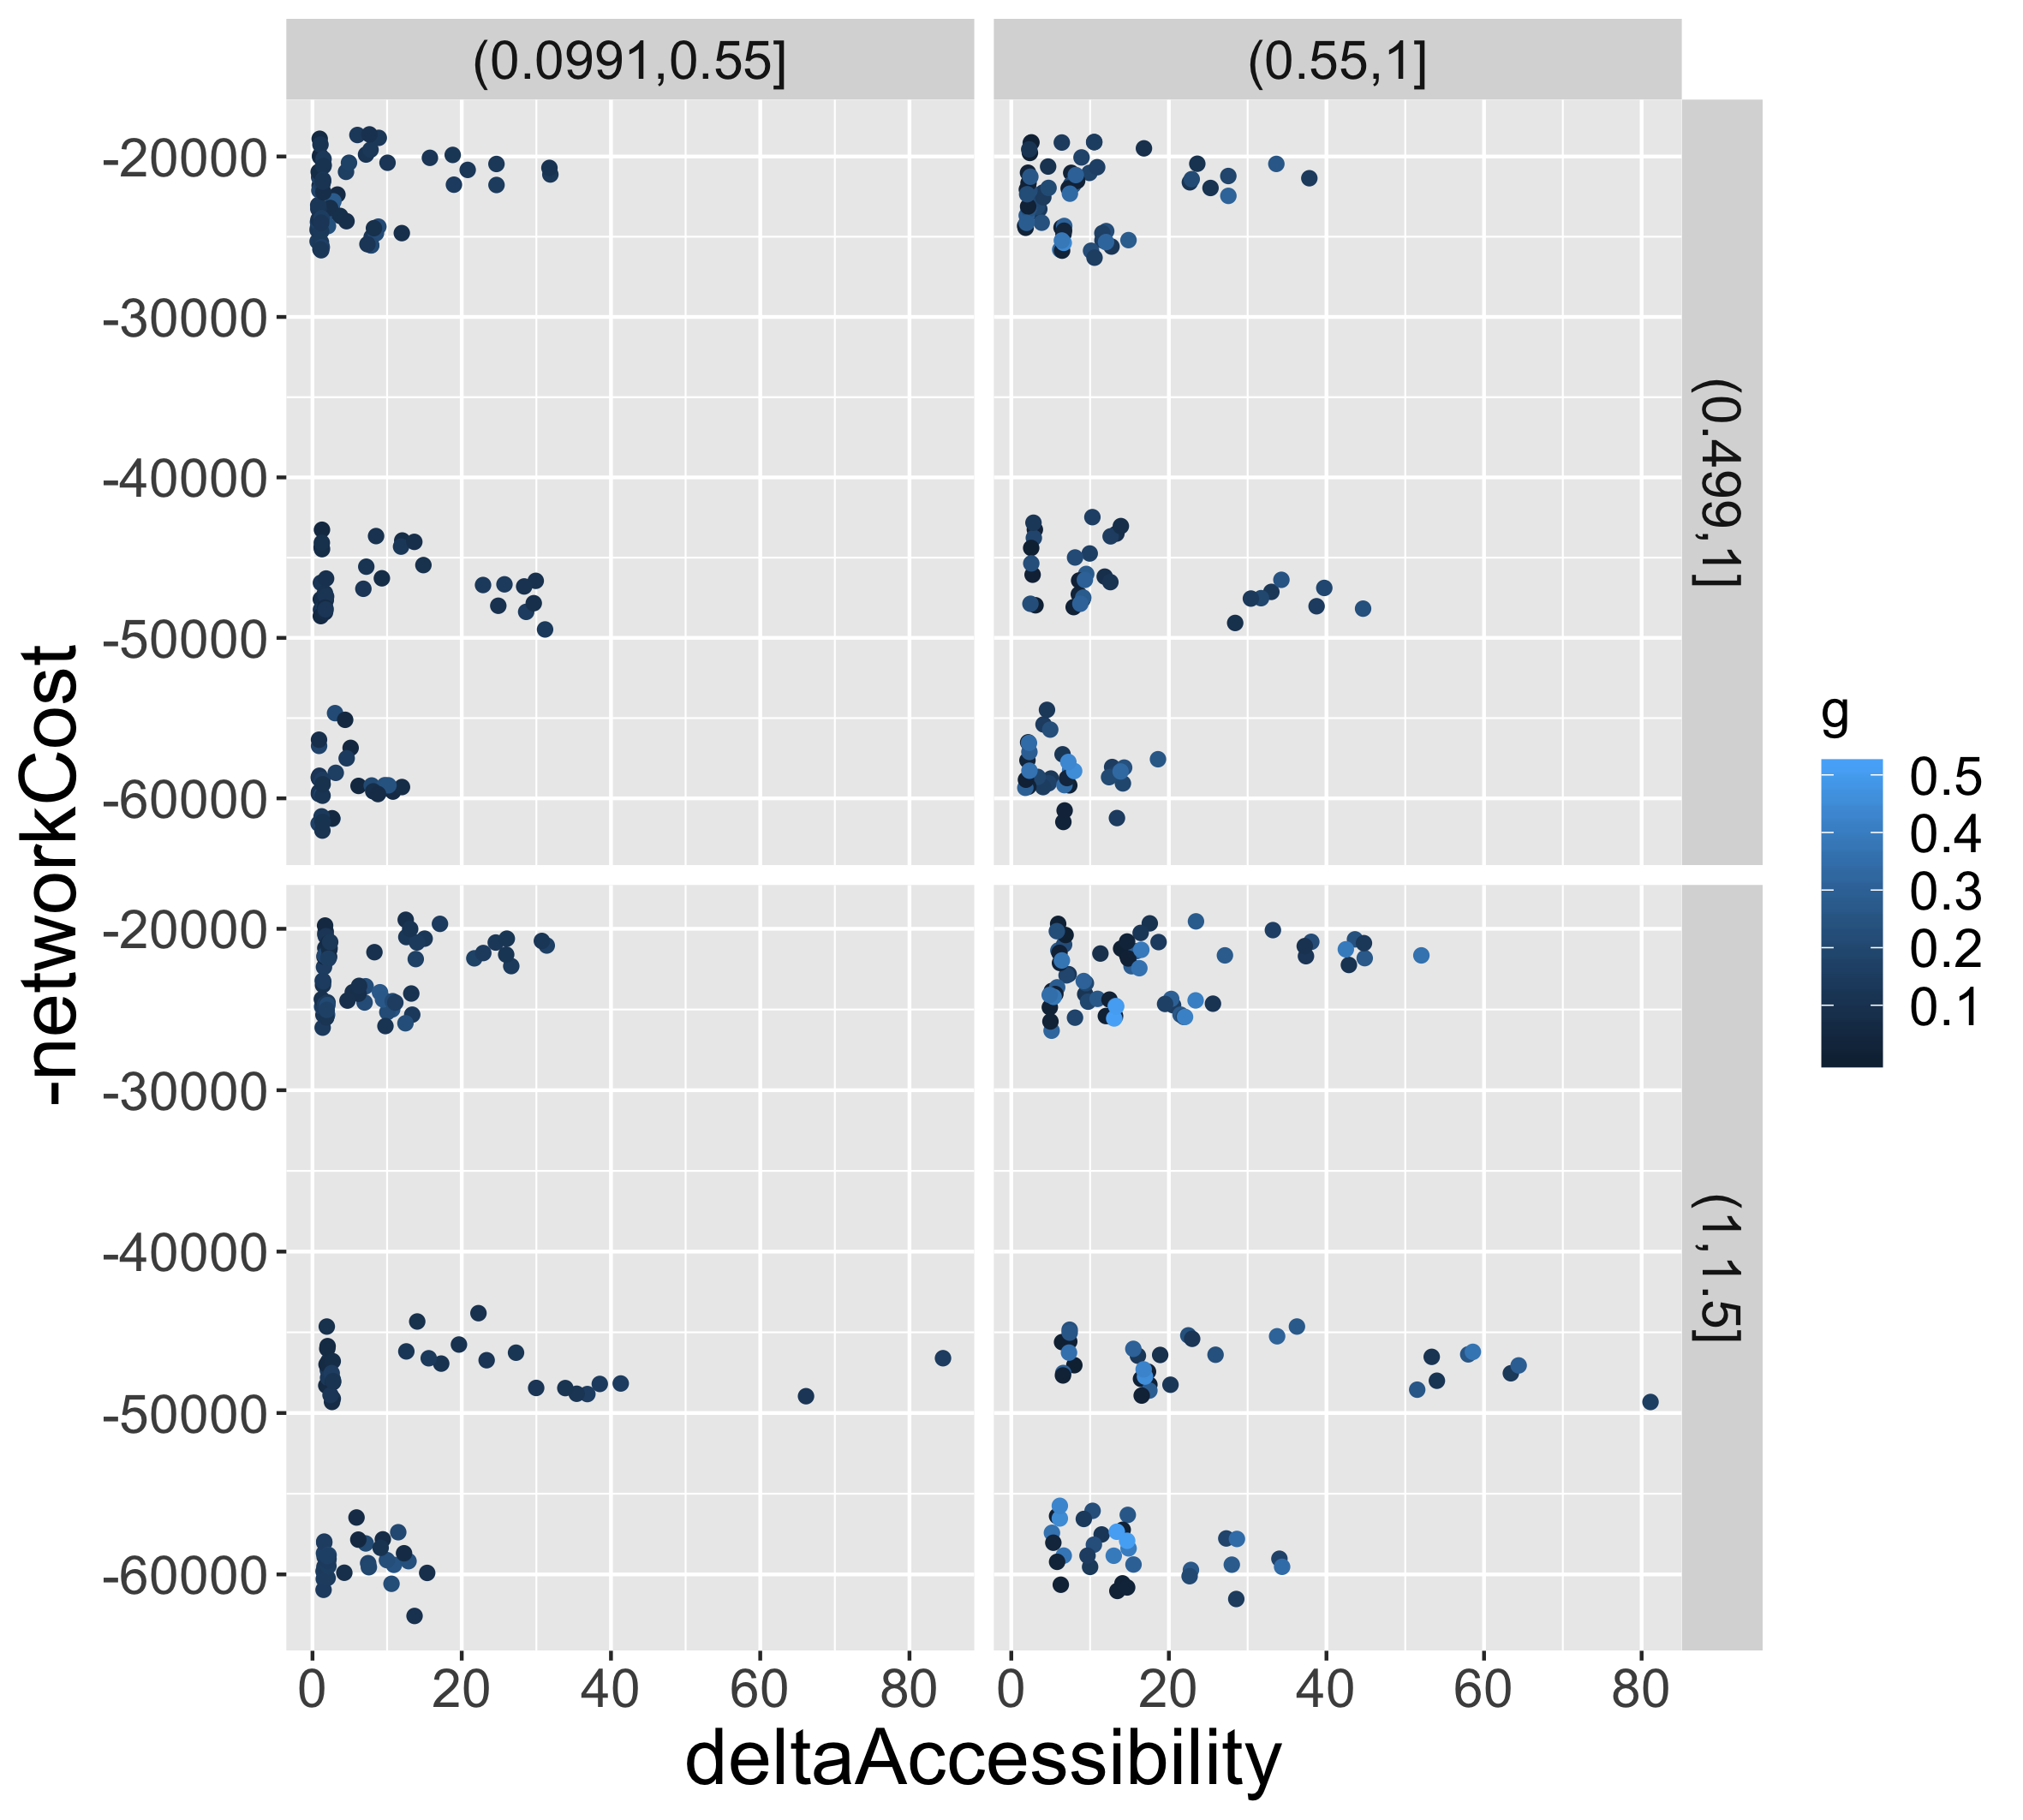
\includegraphics[height=0.65\textheight,width=0.65\textwidth]{figures/pareto-access-cost_cut2.png}	
%\end{figure}

%{\footnotesize Rows: hierarchy; columns: $c_0$}

\textit{Intermediate values of governance levels on the optimal Pareto front when international exchanges are intense (right column)}




%\sframe{Role of urban hierarchy}{
% We also show that initial spatial conditions such as urban hierarchy significantly influence model outcomes [5].
% -> GSA
%}


\section{Discussion}



% This work illustrates how co-evolution models at this scale can be refined, opening research possibilities towards more complex or multi-scale models.

% Discuss alternative flow assignment procedures. You can in particular have a look at the transportation literature

% Discuss the structure of this model, of canonical LUTI, and of a sample of more advanced LUTI models could a much more detailed representation of underlying capture intrinsic crucial process which would be missed by our approach? In other words, what is the purpose of LUTI models? More generally, discuss the relation between the degree of validation of a model and its potential operationalization.


% game type - Nash eq?


\textbf{Developments}

Towards a macroscopic Land-use Transport model (including other network assignment procedures and congestion)

More elaborated representation of decision-making and governance processes


Integration into a multi-scale model \cite{raimbault:halshs-02351722}


\textbf{Applications}

Evaluate transportation scenarios/projects in a multinational stakeholders context


Planning for sustainable territories on long time scales











\section{Conclusion}

A co-evolution model at the macroscopic scale complexified by including transportation governance

Well understood stylized models as a first step towards policy applications



\textbf{Open repositories}

\url{https://github.com/JusteRaimbault/CoevolGov} for the model

\url{https://github.com/JusteRaimbault/Governance} for results


\bigskip

\textbf{Simulation data at} \url{https://doi.org/10.7910/DVN/WP4V7S}





\bibliographystyle{unsrt}
\bibliography{biblio}


% Appendices?

%% possible questions?
%% application to real systems?
%% policy applications?
%% def/carac coevol
%% multiscale? ~
%
%}
%
%
%\sframe{Defining co-evolution}{
%
%}
%
%\sframe{Characterizing co-evolution}{
%
%}
%
%\sframe{A LUTI model with governance processes}{
%
%}







%\appendix




\end{document}


%%%
% template
%
%\begin{table}
%\caption{\label{jlab1}Journals to which this document applies, and macros for the abbreviated journal names in {\tt iopart.cls}. Macros for other journal titles are listed in appendix\,A.}
%\footnotesize
%\begin{tabular}{@{}llll}
%\br
%Short form of journal title&Macro name&Short form of journal title&Macro name\\
%\mr
%2D Mater.&\verb"\TDM"&Mater. Res. Express&\verb"\MRE"\\
%Metrologia&\verb"\MET"&Transl. Mater. Res.&\verb"\TMR"\\
%\br
%\end{tabular}\\
%$^{a}$UK spelling is required; $^{b}$MSC classification numbers are required; $^{c}$titles of articles are required in journal references; $^{d}$Harvard-style references must be used (see section \ref{except}); $^{e}$final page numbers of articles are required in journal references.
%
%\end{table}
%\normalsize
%
%
%\subsection{Inclusion of graphics files\label{figinc}}
%Using the \verb"graphicx" package graphics files can 
%be included within figure and center environments at an 
%appropriate point within the text using code such as:
%\small\begin{verbatim}
%\includegraphics{file.eps}
%\end{verbatim}\normalsize
%The \verb"graphicx" package supports various optional arguments
%to control the appearance of the figure. Other similar 
%packages can also be used (e.g. \verb"graphics", \verb"epsf").   Whatever package you use,
%you must include it explicitly after the \verb"\documentclass" declaration using (say)
%\verb"\usepackage{graphicx}".
%




